\documentclass[sigconf,authorversion,nonacm]{acmart}

\usepackage{minted}
\usepackage{subcaption}
\usepackage{booktabs}
\usepackage{tabularx}

\setminted[python]{fontsize=\small,breaklines}
\renewcommand\tabularxcolumn[1]{m{#1}}

\begin{document}
\title{Project Paper}
\subtitle{Team 4: LDA}

\author{Webi Tesfaye Dabuse}
\authornote{Team Leader}
\affiliation{
    \institution{KAIST}
    \city{Daejeon}
    \country{South Korea}
}
\email{webby@kaist.ac.kr}

\author{Melka Dawit Legesse}
\affiliation{
    \institution{KAIST}
    \city{Daejeon}
    \country{South Korea}
}
\email{kaidavid7@kaist.ac.kr}

\author{Ohjun Kwon}
\affiliation{
    \institution{KAIST}
    \city{Daejeon}
    \country{South Korea}
}
\email{ohjun@kaist.ac.kr}

\begin{abstract}
    Our project focuses on implementing the text mining concepts and techniques we have learnt in our CS474 - Text Mining class. Queries such as ‘Top 10’ or ‘Best 10’ are one of the most common search phrases. As a result, we aim to extract the top 10 most significant issues that happened over a certain timeframe  and events that are both significantly and indirectly tied to them by looking at Korea news articles reported over a three years period - 2015, 2016, and 2017.

    We implemented k-means, DBSCAN clustering techniques, document level relation extraction with spacy and stanza, dimensionality reduction with PCA and UMAP, cosine-based document similarity, topic modelling using BERTopic and embedding with different pretrained models.

    You can download our project source from here\footnote{https://github.com/webby64/CS474\_project}.
\end{abstract}

\maketitle
\section{Introduction}
Text data holds the most part of unstructured data that, by itself,  accounts for 80% of all the existing data, and therefore it is a rich source for data analytics and AI application deployments making Text Mining an essential field. Furthermore, Text Mining draws upon several related fields such as IR, Data Mining, NLP, and others. Its aim of automatically identifying patterns within raw text are achieved through text/ document categorization, summarization, clustering, sentiment analysis, entity relation modeling and so on.

The first step of any Text Mining process is data gathering followed by understanding and preprocessing the gathered data before jumping to its analysis.

\section{Problem Definition}
As news agencies continuously report what happens across the globe, they are great sources of text data. Their articles can be used to extract the most trending issues for a given time interval and to track some events by applying different Text Mining techniques. In this term project, we will be relying on Korean newspaper articles to accomplish these tasks.

Keywords: Clustering, PCA, Relation Extraction, Cosine Similarity, BERTopic, RoBERTa, Topic Modelling

\subsection{Clustering}
An unsupervised machine learning approach for grouping documents based on the similarity of the  information they possess. The vector based clustering methods: K-means and DBSCAN - Density Based Spatial Clustering of Applications with Noise clustering are mainly applied in our project. K-means is a centroid-based or partition-based clustering algorithm, whereas DBSCAN is a density-based clustering algorithm favouring densely populated clusters and expectation maximization (EM).

\subsection{Relation Extraction}
The task of relation extraction is an important and challenging task in the field of information extraction (IE). It extracts semantic relationships existing between different entities such as people, places, organizations, dates, currency, and so on. While sentence-level (Intra-sentence) relationships are comparably easy to extract, document-level (Inter-sentence) relationship extraction is cumbersome as it aims to extract relations among multiple entity pairs of a document.For this purpose, pretrain models are used for embedding and Spacy is used for entity recognition without constructing semantic categories between entities.

\subsection{Document Similarity}
The distance between two documents can be used as a key factor for information retrieval and the different methods that are implemented are: Jaccard distance, Cosine distance, Euclidean distance, and Relaxed Word Mover’s distance with Cosine and Euclidean being the most common and effective for documents represented in vector space. Additionally, the different embedding techniques that are used to represent a document as a vector are: Tf-Idf, Word2Vec, GloVe, Doc2Vec, and BERT.

\section{Issue Trend Analysis}

This task is to rank the top ten most significant issues
that have been observed in the given news dataset
which includes news articles of three years(2015-2017).

\begin{figure}[ht]
    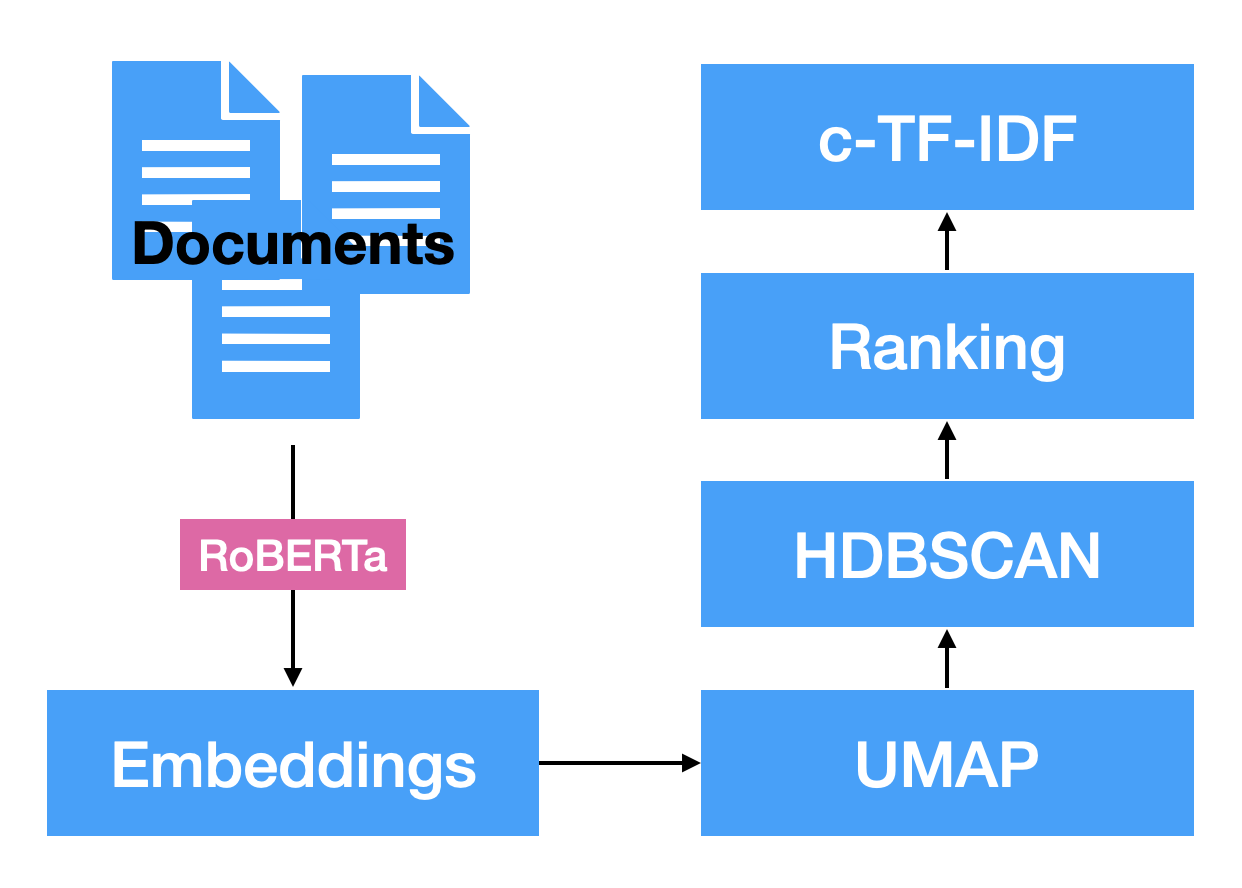
\includegraphics[width=0.6\linewidth]{img/process.png}
    \caption{Overall pipeline}
    \label{fig:process}
\end{figure}

In order to select the top ten most significant issues,
we need to first identify what issues are referenced by the articles.
Identifing issues is possible by grouping simliar articles and extract several
important keywords which differenciate a group of articles from the others.
We can collect simliar articles by embedding articles into some vector space
using a language model, and running a unsupervised clustering algorithm on them.
After that, we can calculate some keywords which can represent those group of article
to name it.
For selecting significant issues, we need to define what issue is considered as
a significant issue.
As discussed in the design paper, let's define a significant issue as an issue
which has lots of related articles within a specific time frame.

\subsection{Document Embedding}
\label{sec:embed}
Firstly, we need to embed the given articles into a vector space.
There were several pre-trained language models avaliable to use as described in Figure~\ref{fig:avail}.
Among available pre-trained language models, we choosed RoBERTa(\mintinline{python}{'all-roberta-large-v1'})
to embed the article.
We have used \mintinline{text}{sentence_transformers} framework to use the pretrained RoBERTa large model.
Embedding documents with this framework is very simple as Listing~\ref{lst:embed}.

\begin{figure}[ht]
    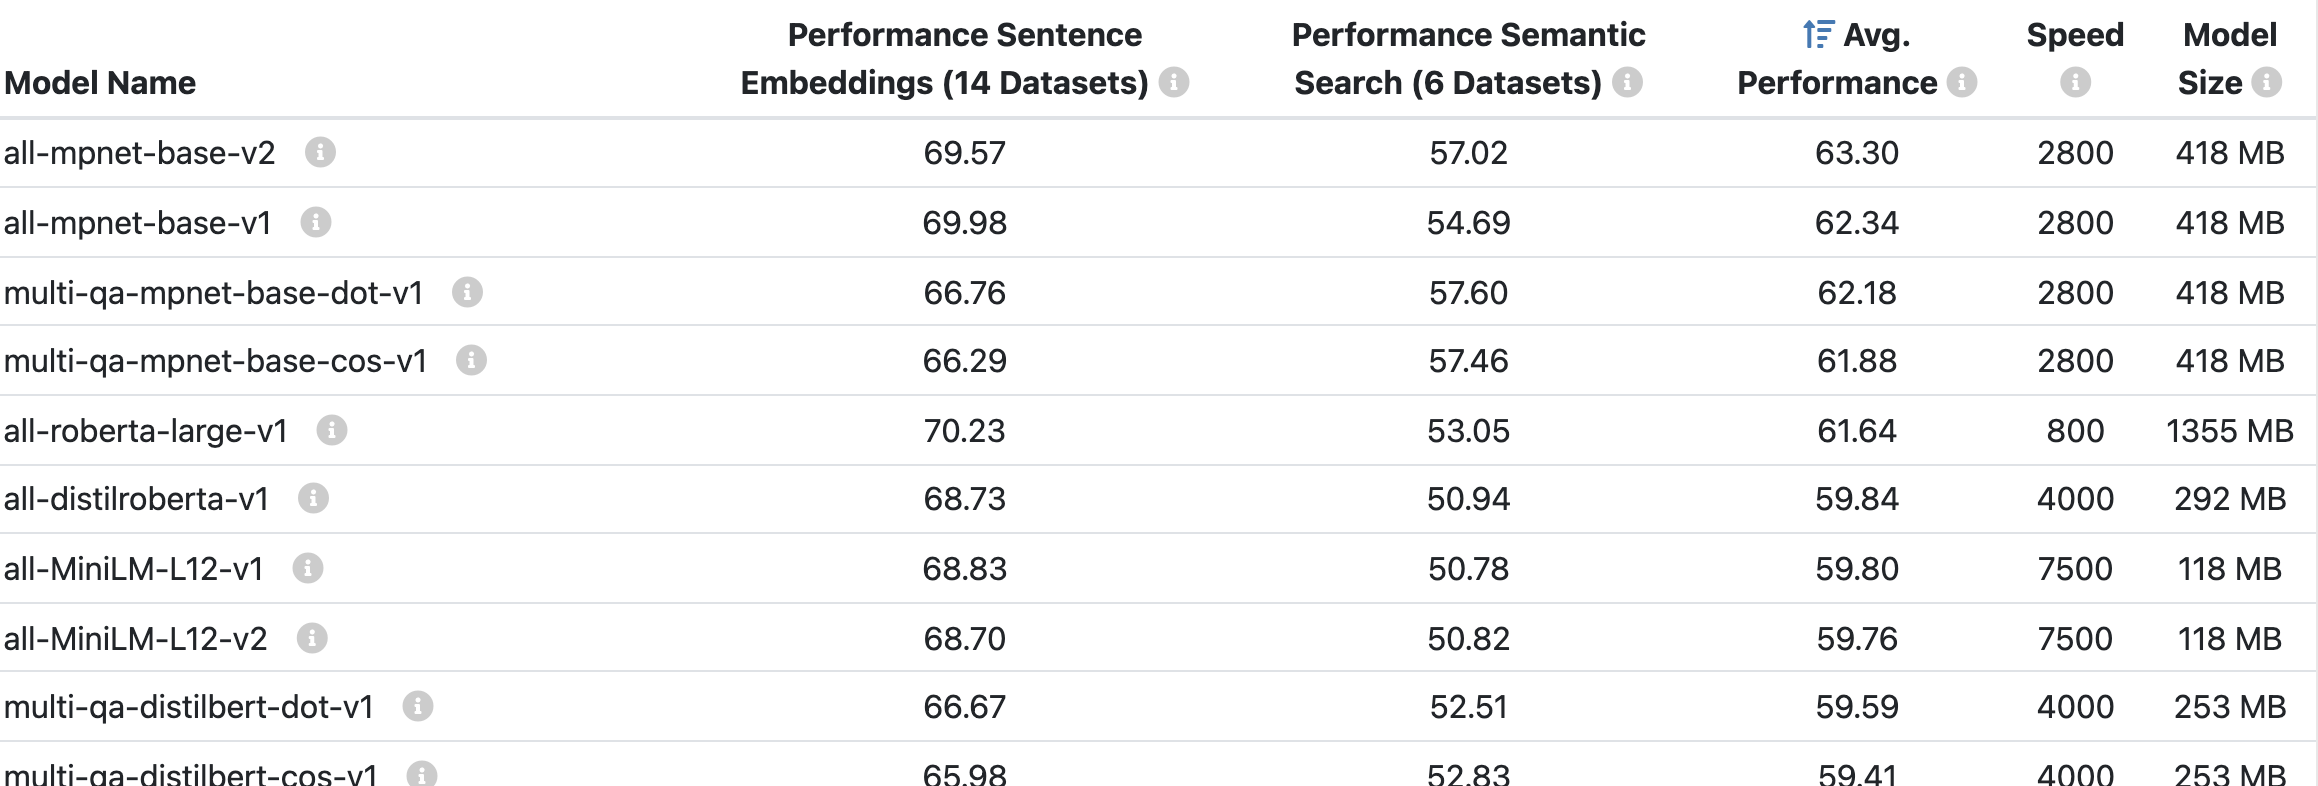
\includegraphics[width=\linewidth]{img/avail.png}
    \caption{Avaliable pre-trained models}
    \label{fig:avail}
\end{figure}

\begin{listing}[ht]
\begin{minted}{python}
from sentence_transformers import SentenceTransformer

model = SentenceTransformer('all-roberta-large-v1')
embeddings = model.encode(docs)
\end{minted}
\caption{Embedding documents with RoBERTa-large model}
\label{lst:embed}
\end{listing}

\subsection{Document Clustering}
\subsubsection{Dimensionality Reduction}
Clustering models are prone to the curse of dimensionality, so
it is better to maintain dimension slim. It also benefits the speed of
calculations.
For dimensionality reduction of the embeddings,
we used Uniform Manifold Approximation and Projection(UMAP).
We have used UMAP as shown in Listing~\ref{lst:umap}

\begin{listing}[ht]
\begin{minted}{python}
dim_reduction = UMAP(n_components=5, min_dist=0, metric='cosine').fit_transform(embeddings)
\end{minted}
\caption{Feature extraction with UMAP}
\label{lst:umap}
\end{listing}

\paragraph{n\_components}
This argument sets the dimension of the space that embeddings will be embed into.
The default value of this argument is 2,
since it's easiar to visualize with two dimensional data according to the developer team.
However, we are going to manipulate very high dimensional data
and we need some space to preserve relationship between articles.
Therefore, this value have been set to 5.

\paragraph{min\_dist}
This argument sets the effective minimum distance between embedded points.
Smaller values will result in a more clustered/clumped embedding.
We have set this value to 0 because we want to cluster them more strictly.

\paragraph{metric}
This argument sets the metric to use to compute distances in the space.
Since we are handling sparse data, we have set this to use cosine simliarity.

\subsubsection{Clustering}
We have chosed HDBSCAN for clustering our embeddings, since it is one of the
nice performing clustering algorithm. HDBSCAN is density-based and able to
figure out outliers, so it suits for this task and works well with UMAP.
We have clustered our articles with Listing~\ref{lst:clustering}


\begin{listing}[ht]
\begin{minted}{python}
clusterer = HDBSCAN(min_cluster_size=40)
clusterer.fit(dim_reduction)
data['topic'] = clusterer.labels_
data['prob'] = clusterer.probabilities_
\end{minted}
\caption{Clustering documents with HDBSCAN}
\label{lst:clustering}
\end{listing}

\paragraph{min\_cluster\_size}
This argument sets the minimum size of clusters. If this value increases,
the number of cluster decreases. This value was chosen heuristically by looking at
the actual result of clustering.

\subsection{Topic Extraction}
Before ranking the topics, it might be easy to extract each topic first
and proceed to topic ranking, because we need to examine whether
the result of topic ranking is plausible or not which requires knowing the
actual issue.

\paragraph{RoBERTa}
First, we tried the same model as we have used in document embedding(\ref{sec:embed}).
All of the articles in each topic has been concatenated and processed as one document for a topic
like Listing~\ref{lst:group}. Then, each document for a topic is embedded, and
all the n-grams are counted by the \mintinline{python}{CountVectorizer} as shown in Listing~\ref{lst:count}.

\begin{listing}[ht]
\begin{minted}{python}
group = data.groupby('topic', as_index=False)
topics = group.agg({' body': ' '.join})
\end{minted}
\caption{Collecting document by topic and aggregating them}
\label{lst:group}
\end{listing}

\begin{listing}[ht]
\begin{minted}{python}
count_vectorizer = CountVectorizer(ngram_range=(1, 3), preprocessor=partial(preprocess, stem_lemmatize=False))
count = count_vectorizer.fit_transform(topics[' body'])
words = count_vectorizer.get_feature_names_out()
\end{minted}
\caption{Counting all n-grams}
\label{lst:count}
\end{listing}

After getting count and word list, we can also embed those words with RoBERTa model.
Finally, we can calculate distance with document vector and word vector.
We have used cosine simliarity here. Then we can extract words that are
nearest from the document vector.
After all the successful embedding, clustering, and extracting, we can obtain
results like Figure~\ref{fig:bert-extract} for each topic group.

\begin{figure}[ht]
    \begin{subfigure}{0.5\linewidth}
        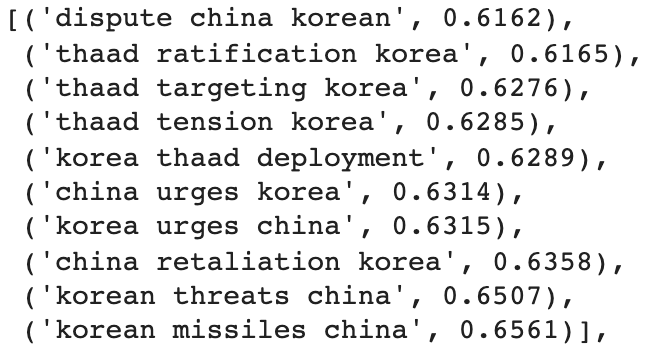
\includegraphics[width=0.9\linewidth]{img/title_bert.png}
    \end{subfigure}%
    \begin{subfigure}{0.5\linewidth}
        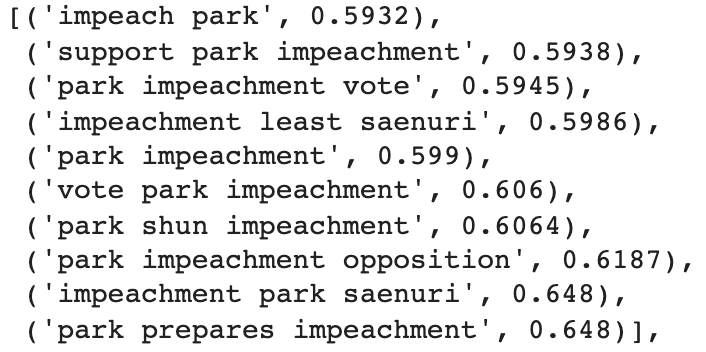
\includegraphics[width=\linewidth]{img/title_bert2.png}
    \end{subfigure}
    \caption{Using RoBERTa to extract topic}
    \label{fig:bert-extract}
\end{figure}

\begin{figure}[ht]
    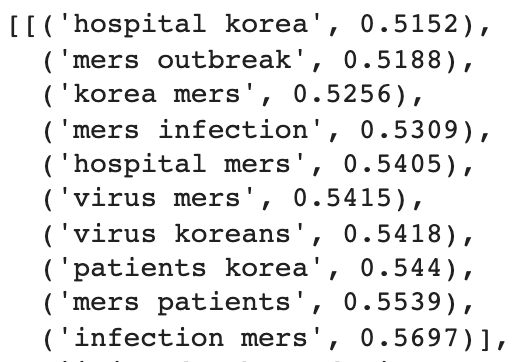
\includegraphics[width=0.5\linewidth]{img/title_bert3.png}
    \caption{Changing n-gram range to 2}
    \label{fig:bert-2}
\end{figure}

\begin{figure}[ht]
    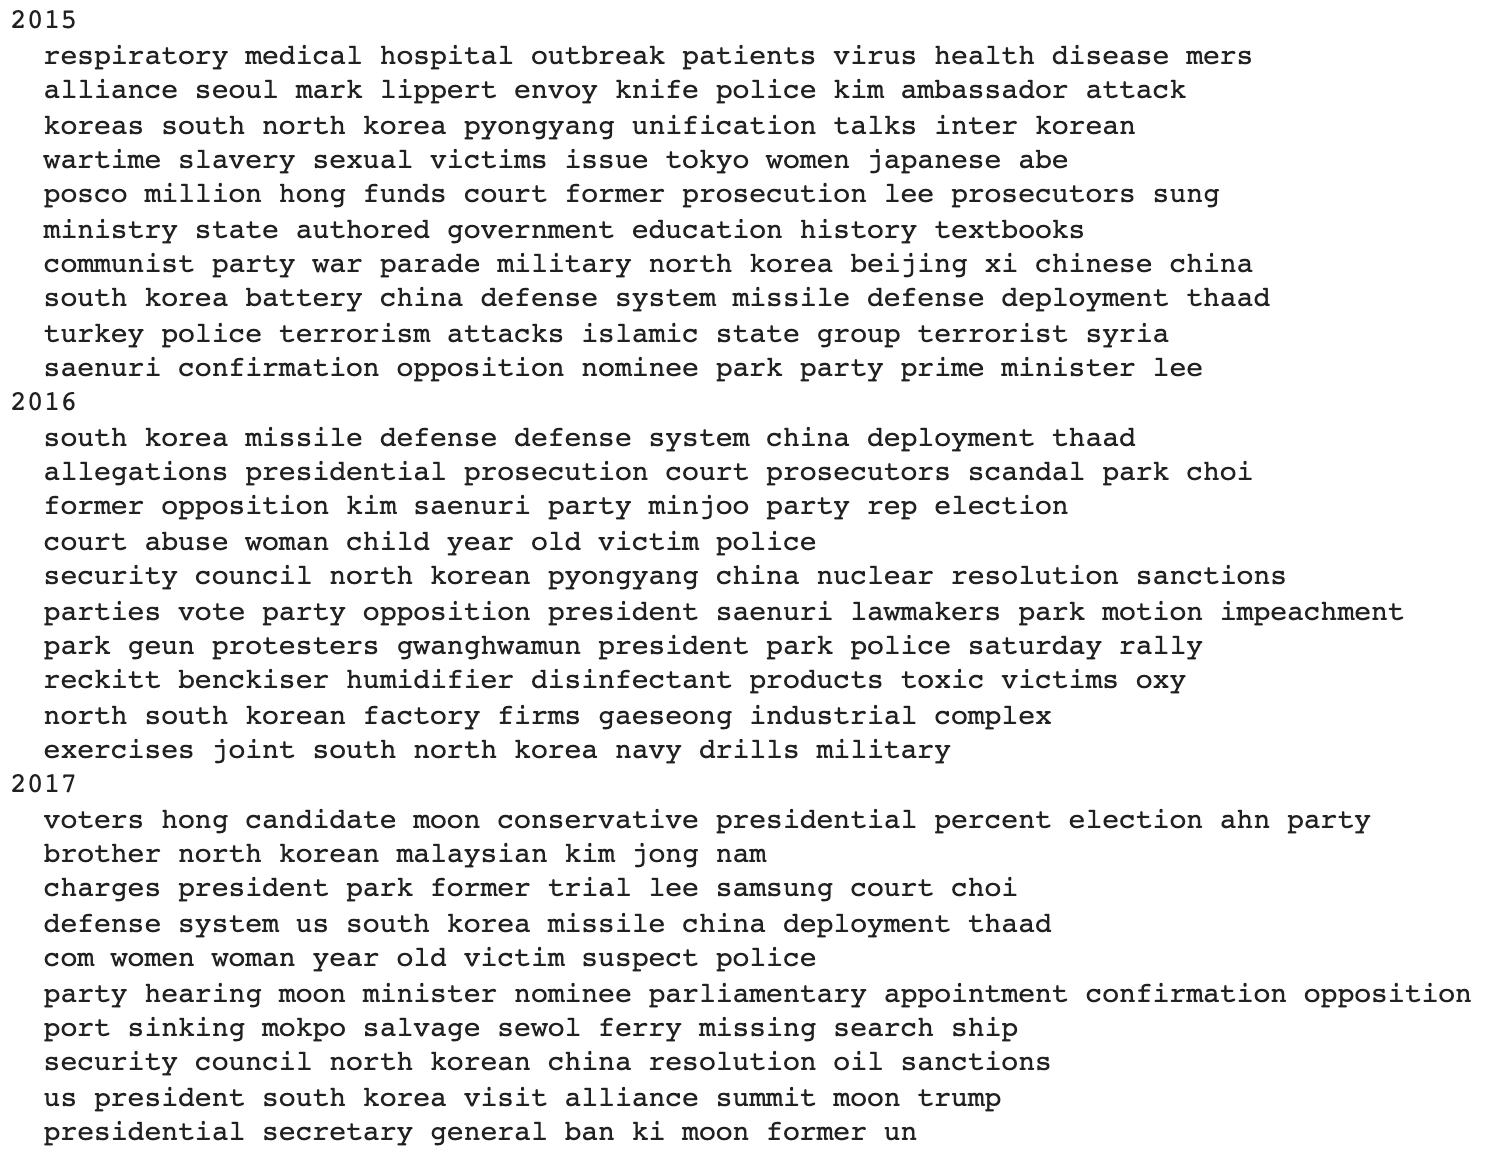
\includegraphics[width=0.9\linewidth]{img/body_ctfidf.png}
    \caption{Using c-TF-IDF to extract topic}
\end{figure}

\subsection{Topic Ranking}
\begin{equation}
    \text{significance} = \max_{i\in[0, 366-d)}\sum^{i+d}_{j=i}j
    \label{eq:sig}
\end{equation}

\begin{listing}[ht]
\begin{minted}{python}
max([sum(days[i:i + length]) for i in range(len(days) - length)])
\end{minted}
\caption{Significance}
\end{listing}


\section{On-issue Event Tracking}
\begin{figure}[ht]
    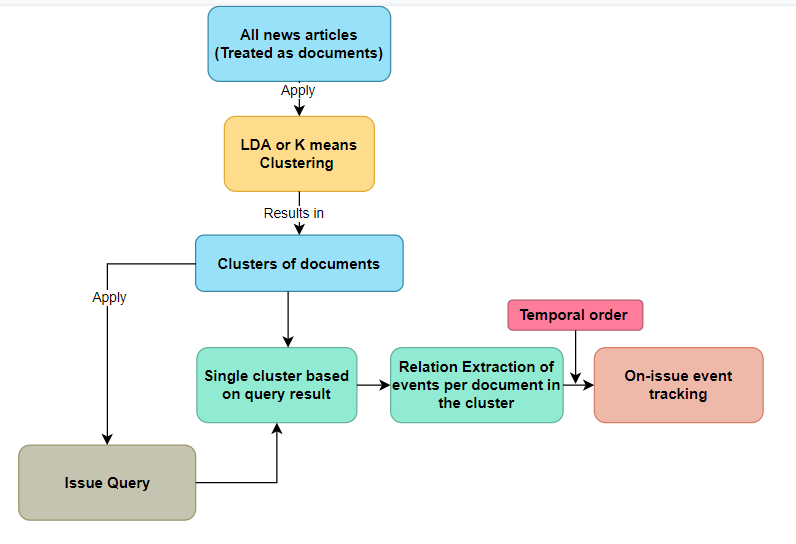
\includegraphics[width=0.9\linewidth]{img/image13.png}
    \caption{Pipeline for task 2-1}
\end{figure}
Event extraction from documents is commonly required for various tasks, such as article summarization, article clustering, and news aggregation. Thus, event extraction is an essential tool in facilitating the categorization and relation between news articles based on the events in their content. This task is implemented to track down events related to two issues from the previous outputs. On-issue events are events that are specifically tied to the issue in question. These events are listed on a temporal line. 

Our approach to tackle this problem starts with clustering the news articles based on their contents. First we used term frequency-inverse document frequency to vectorize the documents so that we can use K-means clustering to categorize these articles into clusters. This approach is unsupervised, therefore, it’s hard to optimize the hyper parameters of the clustering algorithm. Considering the number of articles in the given dataset and their distribution among the clusters we decided to use K-means clustering with k=50. We used the Scikit Learn python library to build this model. This tool provides the center of each cluster so that we can calculate the distance of each vector from its cluster’s center (we will be using this distance in the following steps). 

In order to select one cluster for investigation regarding an issue, we measure the relevance of each cluster to that issue by querying that specific issue inside the articles in each cluster. By querying the issue to each cluster, we collect the significance of each cluster to the issue based on how frequent the issue appeared in the cluster. The most relevant cluster, C, is selected and the articles inside the cluster are further investigated to get on-issue events on a temporal line. 

The center of cluster C is used as a good frame of reference to select the closest vector embedding of an article that is going to be used for event extraction. The vectors inside cluster C are sorted based on their euclidean distance from the center. 10 closest vectors are selected for the event extraction from the articles. After several attempts of using the article body for event and relation extraction (using models such as bertopic, bert-large), we decided to leverage the combined resource of body and title of each article in the top 10 closest vectors category using stanza’s CoreNLPClient and pipeline. 

We use Stanza to annotate the sentences in the selected articles. Stanza pipeline is also used for the task of named entity recognition. Using this library, we identify the Detailed information such as Person, Organization and Place.

\subsection{Results}
Event extraction phase in this task uses the embedding of articles to measure the relation between issue and an event. This resulted in inconsistent events on a temporal line. There have been issues of duplicate events as a result of this.

\begin{figure}[ht]
    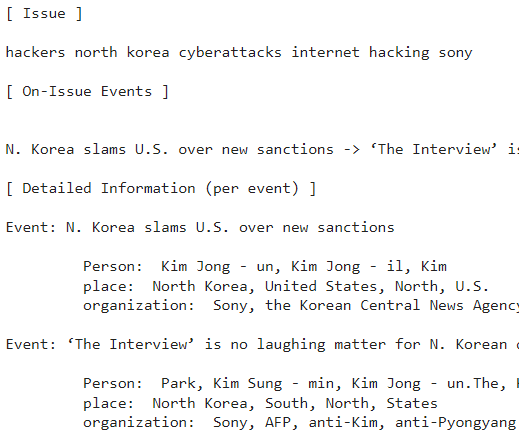
\includegraphics[width=0.8\linewidth]{img/image5.png}
    \caption{Sample output for task 2-1}
\end{figure}

\begin{figure}[ht]
    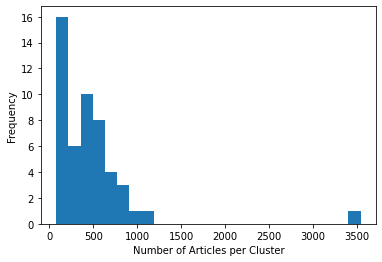
\includegraphics[width=0.8\linewidth]{img/image4.png}
    \caption{Number of articles and their frequency k=50}
\end{figure}

The clustering for task-2 shows that the dataset has a wide range of topics with different number of articles per cluster. One anomalous cluster has 3538 articles. After inspecting most of the articles’ body, we found that several articles are related to North Korea and Crimes in Korea (Social Affairs). This irregularity has not improved with different k values. 


\section{Related-issue Event Tracking}
In our design paper, we mentioned that after finding the top issues of each year and automatically extracting detailed information from two issues which are the most suitable for such analyses, we will be identifying other events that are related to them but not directly tied. Unlike the first task, which looks at articles released within the same year - 2015, 2016, or 2017, in this stage, we will be looking at the entire corpus and mainly rely on clustering.

While performing RE (Relation Extraction) for both on-issue event tracking and related-issue event tracking, we will be extracting factors such as individuals’ names, organizations, and places mentioned within the documents. Our first attempt to use these factors for distinguishing the two tasks was impracticable; however, a satisfactory result was obtained through clustering.

\begin{table}[ht]
    \begin{tabularx}{\linewidth}{>{\centering\arraybackslash}Xcccc}
        \toprule
        & \multicolumn{2}{c}{UMAP} & \multicolumn{2}{c}{PCA} \\
        \cmidrule(lr){2-3}\cmidrule(lr){4-5}
        dimension & 5 & 150 & 5 & 150 \\
        \midrule
        \addlinespace[0.5em]
        all-mpnet-base-v2 & 7m 11s & 25m 31s & 8m 31s & 5m 20s \\
        \addlinespace[0.5em]
        all-roberta-large-v1 & 13m 33s & 31m 57s & 17m 16s & 11m 33s \\
        \addlinespace[0.5em]
        distilbert-base-nli-mean-tokens & 4m 14s & 22m 50s & 4m 6s** & 2m 22s \\
        \addlinespace[0.5em]
        tf-idf & error & 36m 23s & 2m 24s & 1m 14s \\
        \bottomrule
    \end{tabularx}
    \caption{}
\end{table}

Time taken to print 3 related issues each with 3 factors for the top-5 topics.

\begin{figure}[ht]
    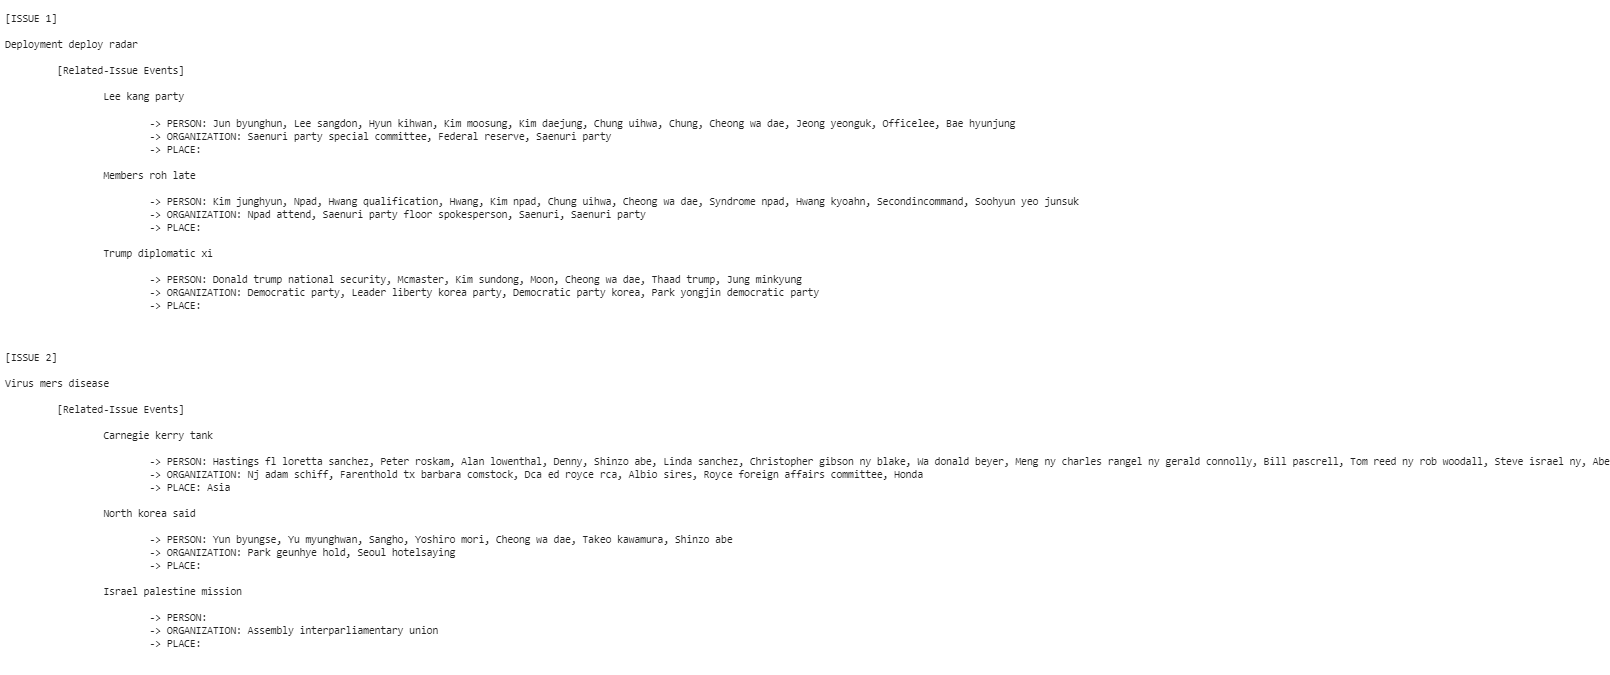
\includegraphics[width=\linewidth]{img/image12.png}
\end{figure}
\begin{figure}[ht]
    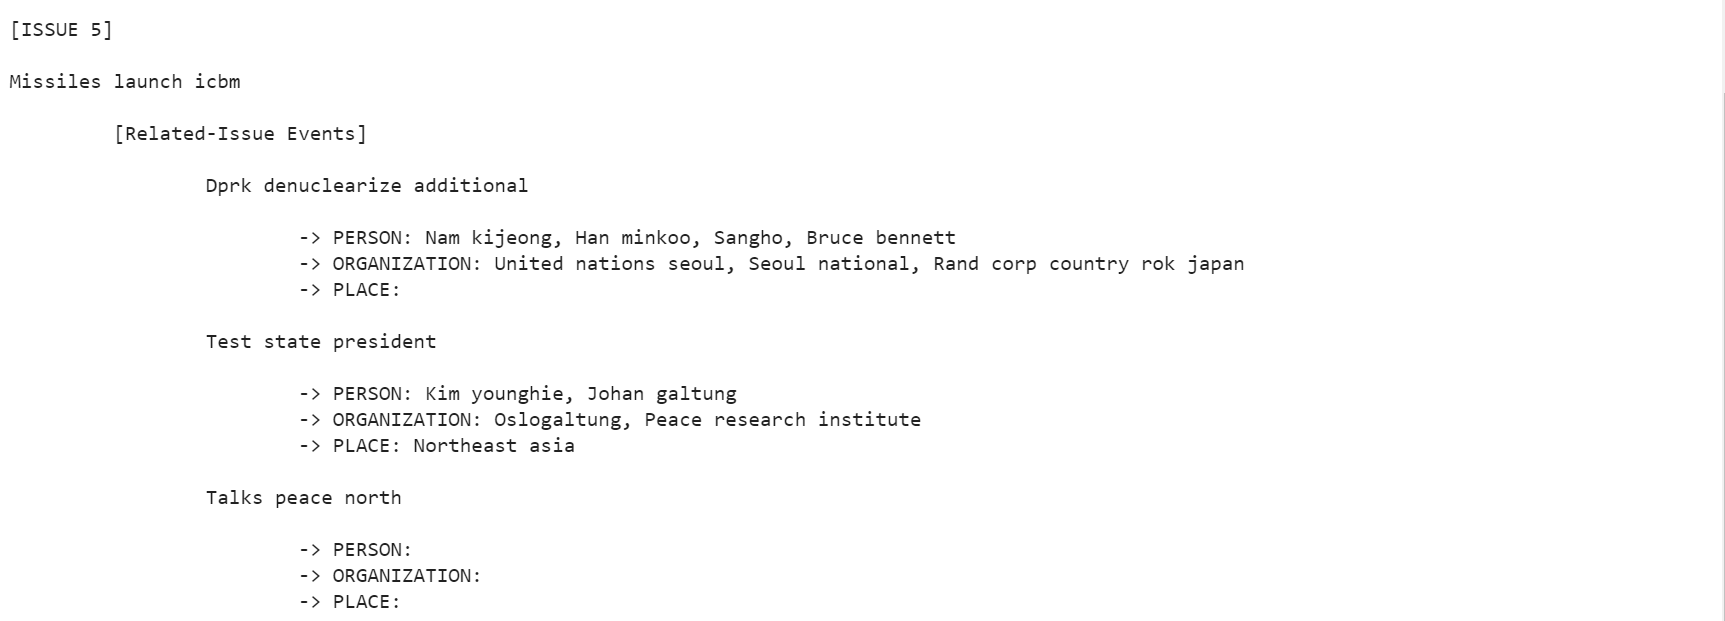
\includegraphics[width=\linewidth]{img/image7.png}
\end{figure}
\begin{figure}[ht]
    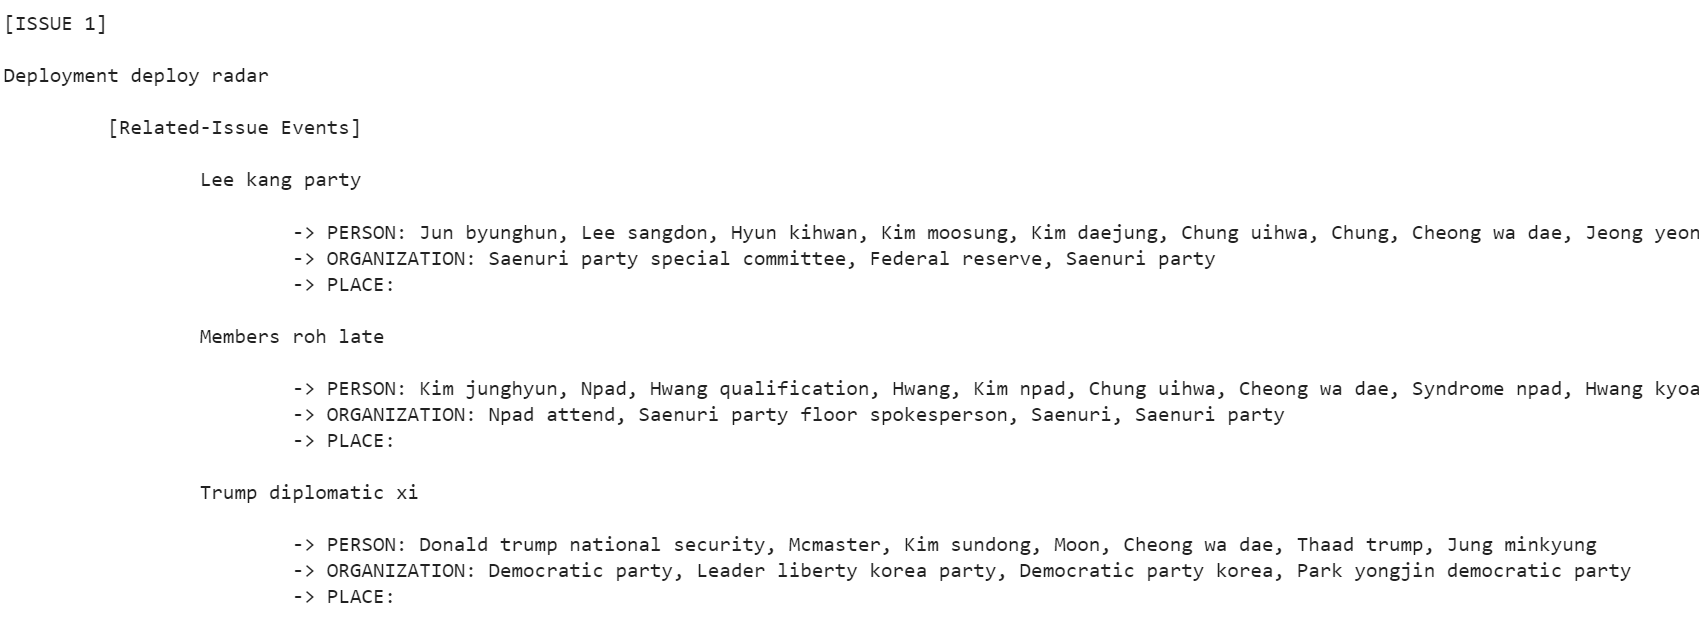
\includegraphics[width=\linewidth]{img/image14.png}
\end{figure}

\subsection{Approaches}
\subsubsection{Clustering}
Cluster the documents by using k-means or dbscan method. Use the document body.
A cluster number of 10 seems sufficient as observed in the elbow method.

\begin{figure}[ht]
    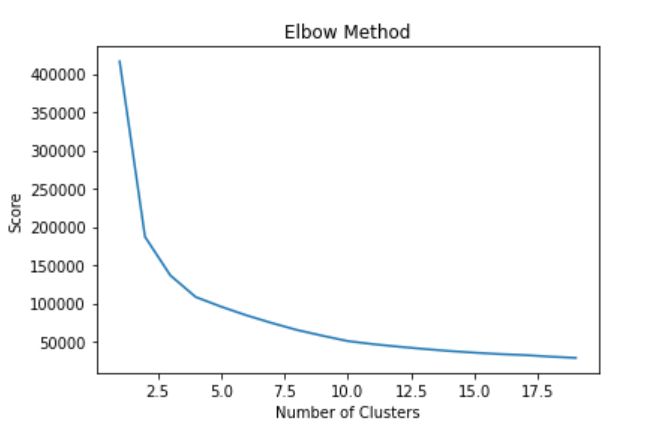
\includegraphics[width=0.7\linewidth]{img/image6.png}
\end{figure}
\begin{figure}[ht]
    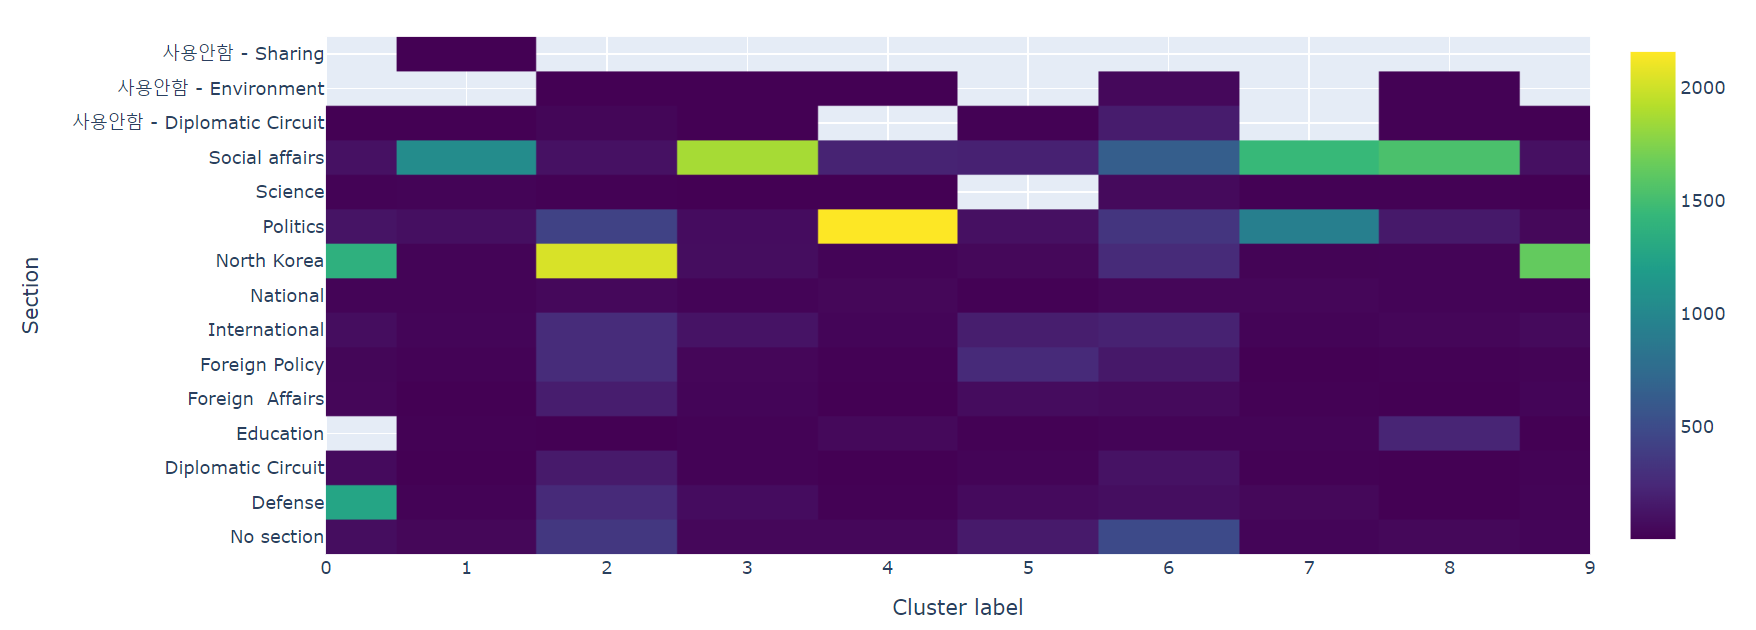
\includegraphics[width=\linewidth]{img/image8.png} 
\end{figure}
\begin{figure}[ht]
    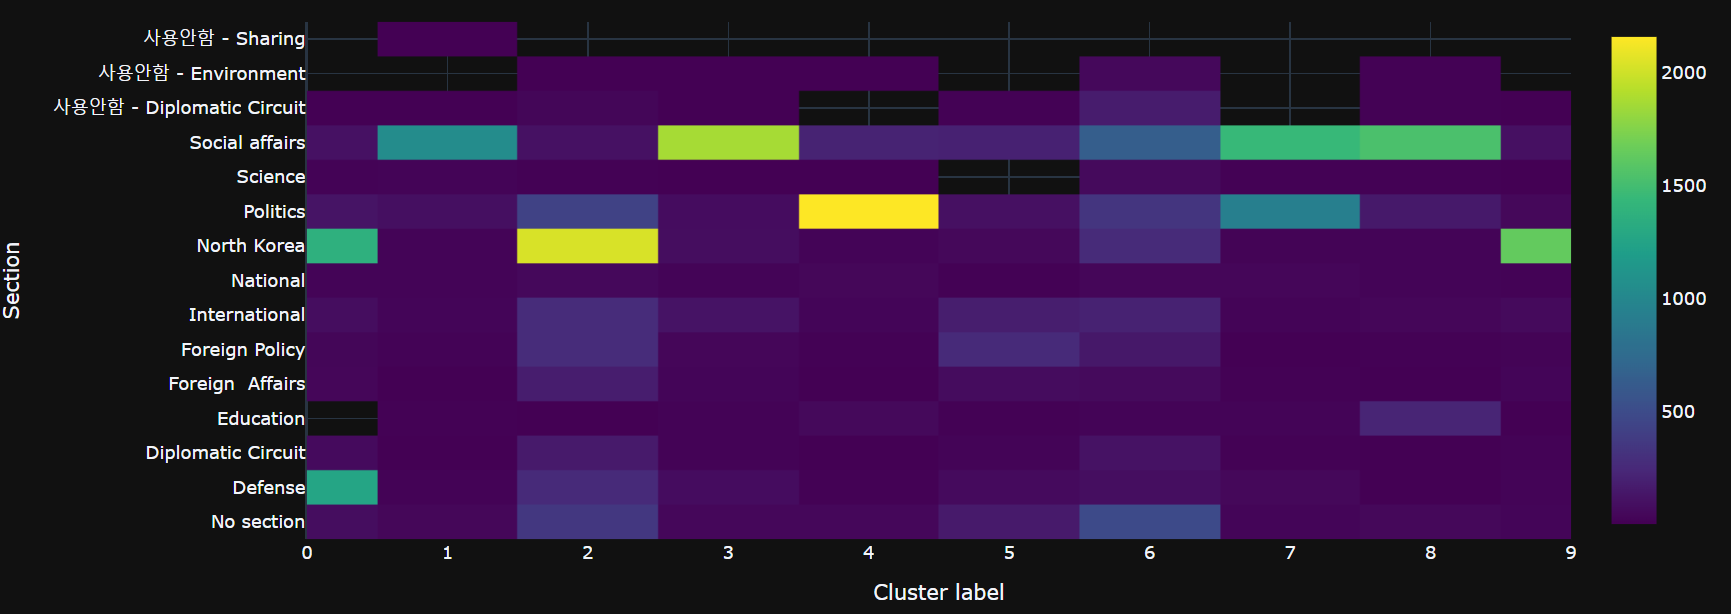
\includegraphics[width=\linewidth]{img/image1.png} 
\end{figure}

The three largest sections: Social affairs, North Korea, and Politics also appear to the largest sections within a cluster.

\subsubsection{Topic Modeling}
Use BERTopic, a topic modeling technique that leverages transformers and c-TF-IDF to create dense clusters along with important topics (issues). Different pretrained models such as all-mpnet-base-v2 and all-MiniLM-L6-v2 are used for embedding the documents. Here, even though the all-MiniLM-L6-v2 model is very fast, we will be using the all-mpnet-base-v2 model as it shows the highest performance on semantic search.

\begin{figure}[ht]
    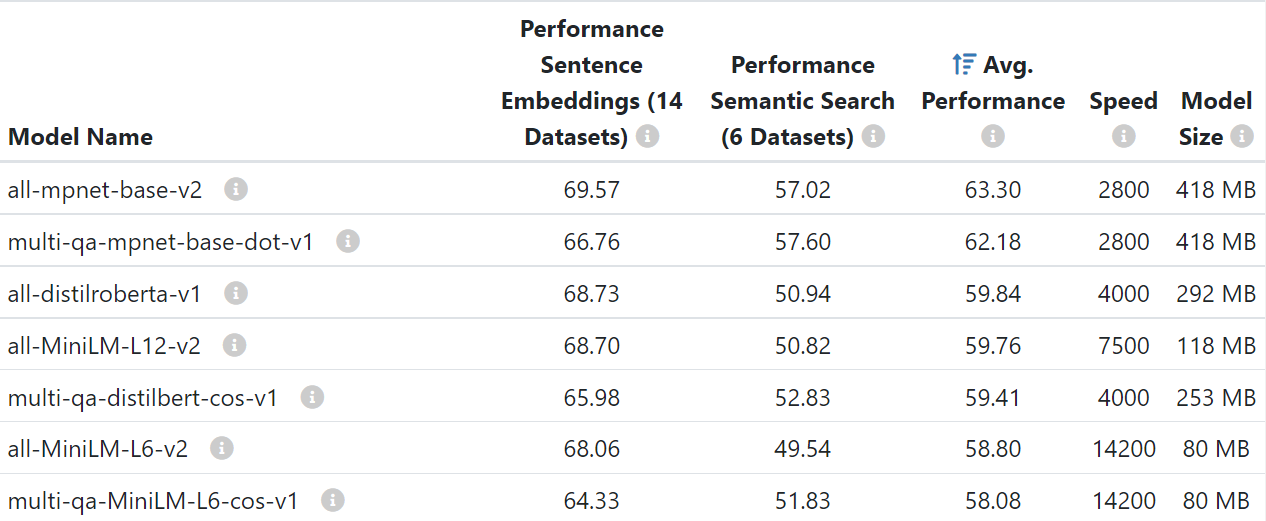
\includegraphics[width=\linewidth]{img/image9.png} 
    \caption{\protect\footnotemark}
\end{figure}

\footnotetext{https://www.sbert.net/docs/pretrained\_models.html}

Afterwards, rely on the cosine similarity between the embedding of the issues obtained from Task-1 (over the 3 years) and the documents in order to rank them from highest to lowest in similarity. This is the same as performing a cosine similarity based query search of the issues over the entire corpus. The number of documents that are the closest to the given issue is a hyperparameter (hyperparameter-2). Furthermore, move into the cluster most of these documents belong to.

This approach is taken to maximize the chance of finding the right cluster the issue belongs to.

\begin{figure}[ht]
    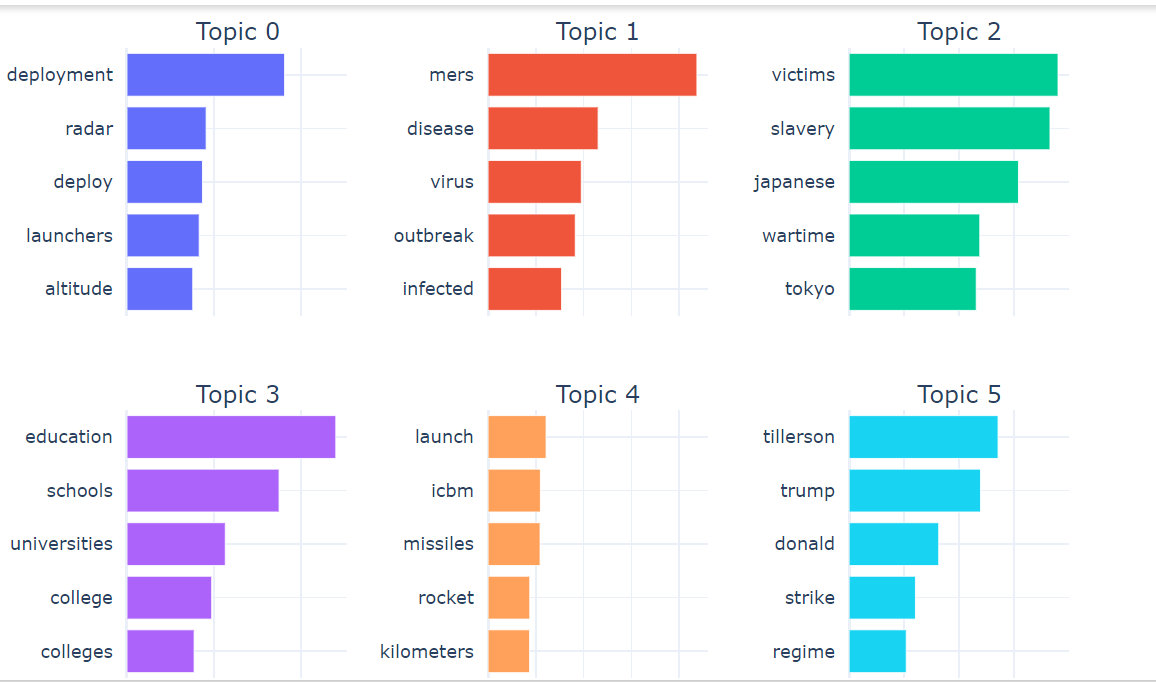
\includegraphics[width=\linewidth]{img/image10.png} 
    \caption{BERTopic - Top 6 topics and the words they contain}
\end{figure}

\subsubsection{Move to neighbouring clusters}
\paragraph{Assumption}
Moving to other clusters neighboring the cluster the issue belongs to, we will likely encounter documents that are less related but indirectly related to it. Neighbouring clusters are ranked based on the euclidean distance of their centroids. We decided to look at the first closest cluster (hyperparameter-3) and analyze all the documents within that cluster.

\paragraph{Dimensionality Reduction}
Upon embedding each document, the vector size becomes 768, 768, 1024, and 139696 for mpnet, distilbert, roberta, and Tf-idf, respectively. Therefore, performing dimensionality reduction without losing information is crucial to save computational power and time. Amongst the different techniques - PCA, tSNE, UMAP, and LDA, we used PCA and UMAP for comparison.

UMAP performs faster than PCA and better in complex datasets; however, it is recommended to use both - use PCA followed by UMAP.

\subsubsection{Extract Related Issues}

Arrange the documents in the neighbouring cluster based on their similarity to the given issue and pick every 10th or 15th (hyperparameter-4) document for entity extraction.  Additionally, we relayed on the first few documents (hyperparameter-5) that are ranked immediately under the selected document for topic extraction. It is the extracted topic that is displayed as a related issue. Hence, BERTopic technique is applied here too.

We relayed on Spacy entity extraction to extract and recognize entities such as people, organizations, locations, countries, and dates.

\begin{figure}[ht]
    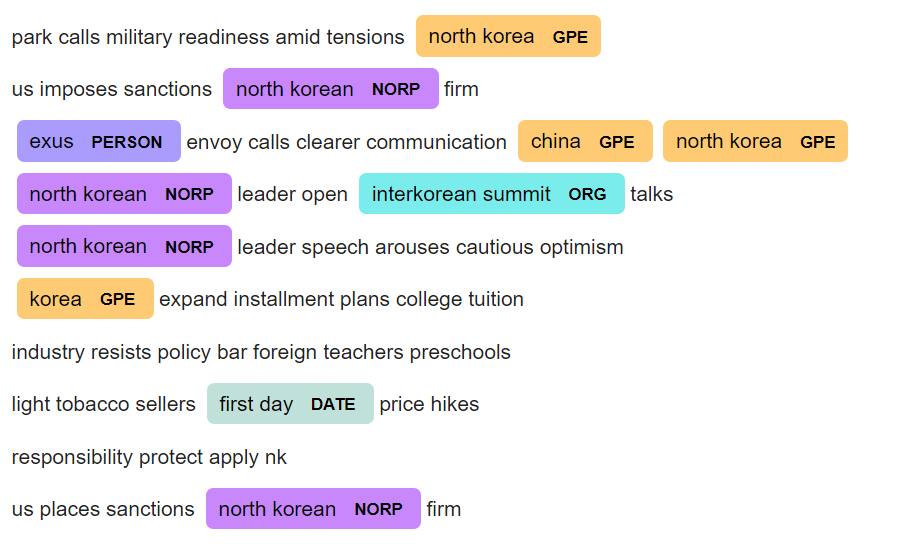
\includegraphics[width=\linewidth]{img/image2.png} 
\end{figure}
\begin{figure}[ht]
    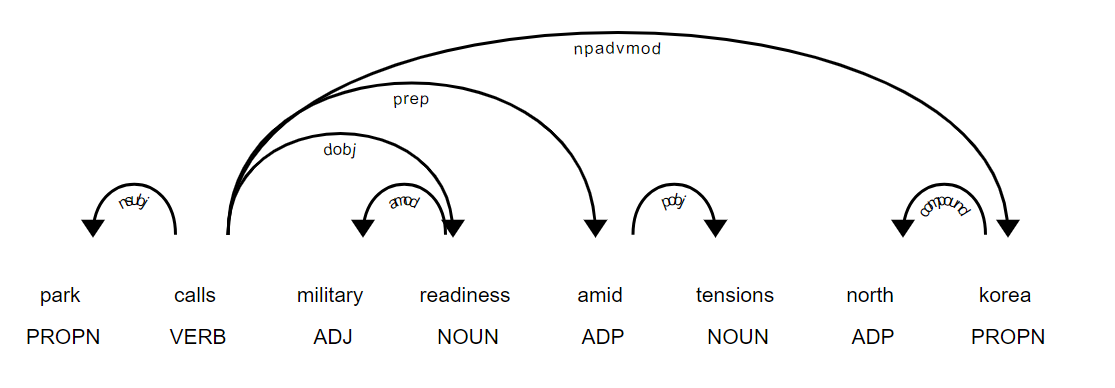
\includegraphics[width=\linewidth]{img/image3.png} 
\end{figure}

\begin{figure}[ht]
    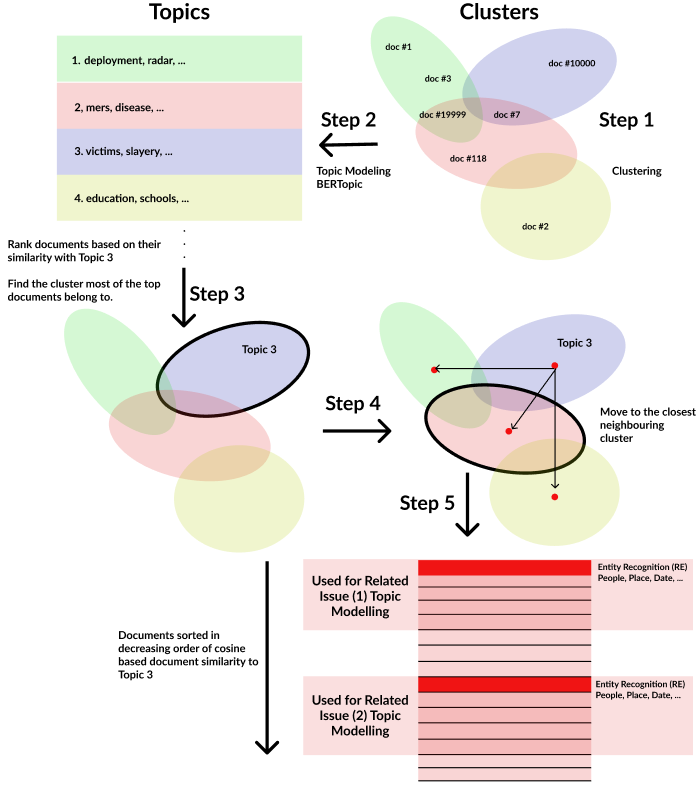
\includegraphics[width=0.8\linewidth]{img/image11.png} 
    \caption{Pipeline}
\end{figure}

\subsubsection{Evaluation}
K-means clustering is evaluated using the elbow method.

Defining a metric value to evaluate the output of each implementation and hyperparameter manipulation was a challenging task, though very necessary for effective optimization. We used our own judgement when changing different hyperparameter values and comparing the outputs.

\nocite{*}
\bibliographystyle{ACM-Reference-Format}
\bibliography{ref}

\end{document}